\documentclass{beamer}
\mode<presentation>
{
	\usetheme{Madrid}

    \definecolor{unisinos}{RGB}{67,40,117}
    \usecolortheme[named=unisinos]{structure}

	\usefonttheme{professionalfonts}
    \usebackgroundtemplate{
\includegraphics[width=\paperwidth,height=0.978\paperheight]{template_unisinos}}

 	\beamertemplatenavigationsymbolsempty
 	\setbeamertemplate{footline}
	{
	  \leavevmode%
	  \hbox{%
	  \begin{beamercolorbox}[wd=.12\paperwidth,ht=2.25ex,dp=1ex,center]{author in head/foot}%
	    \usebeamerfont{author in head/foot}\insertshortauthor
	  \end{beamercolorbox}%
	  \begin{beamercolorbox}[wd=.88\paperwidth,ht=2.25ex,dp=1ex,center]{title in head/foot}%
	    \usebeamerfont{title in head/foot}\insertshorttitle\hspace*{3em}
	    \insertframenumber{} / \inserttotalframenumber\hspace*{1ex}
	  \end{beamercolorbox}}%
	  \vskip0pt%
	}
 	\setbeamertemplate{caption}[numbered]
 	\usepackage{caption}

 	\usepackage[brazil]{babel}		% Idioma do documento
	\usepackage{siunitx}
	\usepackage{ragged2e}
	\usepackage{float}
    \usepackage{indentfirst} }
    \usepackage[alf]{abntex2cite}   % Citações padrão ABNT
	\usepackage{color}			    % Controle das cores
	\usepackage[T1]{fontenc}		% Selecao de codigos de fonte.
	\usepackage{graphicx}			% Inclusão de gráficos
	\usepackage[utf8]{inputenc}		% Codificacao do documento (conversão automática dos acentos)
	\usepackage{txfonts}			% Fontes virtuais

\title[Tópico Especial - Detecção de Fumaça e Chamas]{Tópico Especial - Detecção de Fumaça e Chamas}
\author[Piaia, G. A.]{
	{\fontsize{10}{8}\selectfont \textbf{Aluno:} Guilherme Angelo Piaia} \\
	{\fontsize{10}{8}\selectfont \textbf{Professor}: Cesar Crovato}
}
%\institute[UNISINOS]{UNISINOS - Universidade do Vale do Rio dos Sinos \\ Engenharia de Controle e Automação}

\date{\today}

\begin{document}

%%%%%%%%%%%%%%%%%%%%%%%%%%%%%%%%%%%

\begin{frame}
	\begin{minipage}{1\linewidth}
		\centering
		    \textbf{UNISINOS - Universidade do Vale do Rio dos Sinos} \\ Mestrado Profissional em Engenharia Elétrica
	\end{minipage}
	\titlepage
\end{frame}

%%%%%%%%%%%%%%%%%%%%%%%%%%%%%%%%%%%

\begin{frame}{Sumário}
	\tableofcontents[]
\end{frame}

%%%%%%%%%%%%%%%%%%%%%%%%%%%%%%%%%%%

\section{Introdução}
\begin{frame}{Introdução}
	\begin{itemize}
		\justifying
		\item Este trabalho contem o estudo de artigos dos últimos 15 anos sobre o tema de detecção de fumaça e chamas, com o
		foco em ambientes industriais. Os artigos abaixo, que possuem técnicas diferenciadas, serão apresentados.
		\begin{itemize}
			\justifying
			\item An Early Fire-Detection Method Based on Image Processing (\citeonline{Chen2004a});
			\item A Fast Accumulative Motion Orientation Model Based on Integral Image For Video 
			Smoke Detection (\citeonline{Yuan2008});
			\item Smoke Detection in Video (\citeonline{Kim2009});
			\item Convolutional Neural Network for Video Fire and Smoke Detection (\citeonline{Frizzi2016});
			\item Smoke Detection Based on Image Processing by Using Grey and Transparency Features (\citeonline{Mutar2018});
		\end{itemize}
	\end{itemize}
\end{frame}

%%%%%%%%%%%%%%%%%%%%%%%%%%%%%%%%%%%

\section{\citeonline{Chen2004a}}

\begin{frame}{\citeonline{Chen2004a}}
\begin{columns}
    \begin{column}{0.50\textwidth}
		\begin{itemize}
			\item \textbf{An Early Fire-Detection Method Based on Image Processing};
			\item Sistema com o objetivo de se detectar o fogo logo no início;
			\item Análise cromática para detecção de chamas;
		\end{itemize}
    \end{column}

    \begin{column}{0.5\textwidth}
		\begin{figure}[H]
		    \centering
		    \begin{center}
		    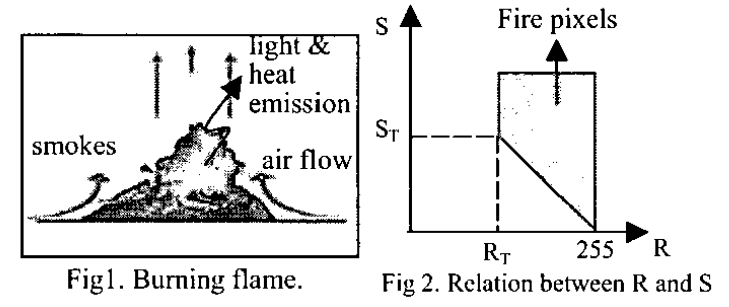
\includegraphics[width=\textwidth]{img/fig1-artigo1.png}
		  \caption{Chama e a relação entre R (\textit{red}) e S (\textit{saturation}).}
		    \label{fig:sar}
		  \end{center}
		\end{figure}
    \end{column}
\end{columns}
\end{frame}

%%%%%%%%%%%%%%%%%%%%%%%%%%%%%%%%%%%

\begin{frame}{\citeonline{Chen2004a}}
\begin{columns}
    \begin{column}{0.50\textwidth}
		\begin{itemize}
			\item Pseudocódigo:
			\begin{gather}
				rule 1: R>R_r \\
				rule 2: R \geq G > B \\
				rule 3: S \geq ((255-R)*S_t/R_t) \\
				IF (rule 1) AND (rule 2) \\
				\quad AND (rule 3) = TRUE \\
				THEN fire-pixel \\
				ELSE not fire-pixel 
			\end{gather} 
		\end{itemize}
		
    \end{column}

    \begin{column}{0.5\textwidth}
		\begin{figure}[H]
		    \centering
		    \begin{center}
		    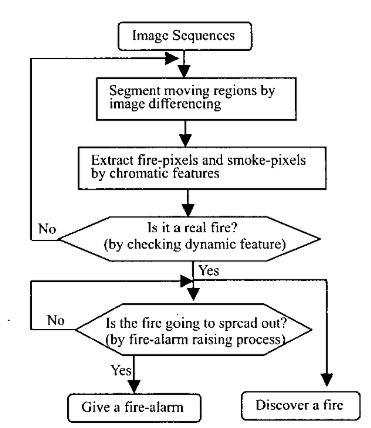
\includegraphics[width=0.8\textwidth]{img/fig5-artigo1.png}
		  \caption{Algoritmo proposto.}
		    \label{fig:sar}
		  \end{center}
		\end{figure}
    \end{column}
\end{columns}
\end{frame}


%%%%%%%%%%%%%%%%%%%%%%%%%%%%%%%%%%%

\section{\citeonline{Yuan2008}}

\begin{frame}{\citeonline{Yuan2008}}
\begin{columns}
    \begin{column}{0.50\textwidth}
		\begin{itemize}
			\item \textbf{A Fast Accumulative Motion Orientation Model Based on Integral Image for Video 
			Smoke Detection};
			\item Proposta de um modelo acumulativo de movimento;
			\item Proposta com o objetivo de melhorar a acurácia da detecção, eliminando 
			falsos positivos;
		\end{itemize}
    \end{column}

    \begin{column}{0.5\textwidth}
		\begin{figure}[H]
		    \centering
		    \begin{center}
		    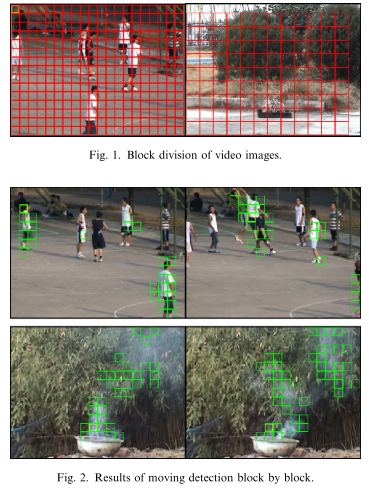
\includegraphics[width=0.7\textwidth]{img/fig2-artigo2.png}
		  \caption{Divisão da imagem em quadros e a detecção do movimento.}
		    \label{fig:sar}
		  \end{center}
		\end{figure}
    \end{column}
\end{columns}
\end{frame}

%%%%%%%%%%%%%%%%%%%%%%%%%%%%%%%%%%%

\begin{frame}{\citeonline{Yuan2008}}
	\begin{figure}[H]
		\centering
		\begin{center}
		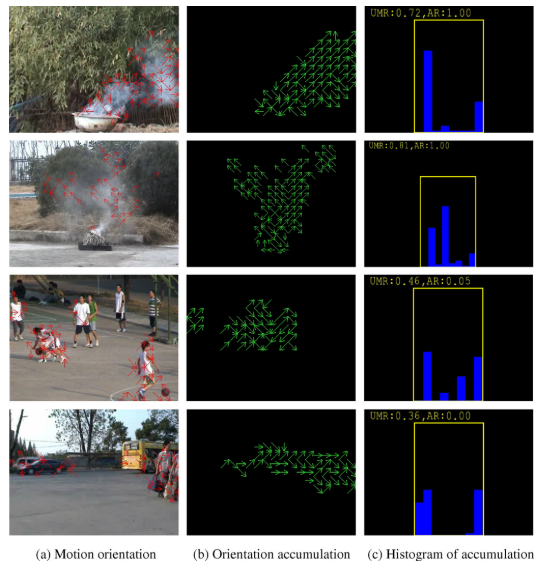
\includegraphics[width=0.52\textwidth]{img/fig7-artigo2.png}
		\caption{Resultados.}
		\label{fig:sar}
		\end{center}
	\end{figure}
\end{frame}

%%%%%%%%%%%%%%%%%%%%%%%%%%%%%%%%%%%

\section{\citeonline{Kim2009}}

\begin{frame}{\citeonline{Han2009}}
\begin{columns}
    \begin{column}{0.40\textwidth}
		\begin{itemize}
			\item \textbf{Smoke Detection in Video};
			\item Proposta que é capaz de diferenciar se a câmera está em movimento, ou
			se há movimento ao fundo;
			\item Proposta para detecção de focos de incêndio em florestas;
		\end{itemize}
    \end{column}

    \begin{column}{0.6\textwidth}
		\begin{figure}[H]
		    \centering
		    \begin{center}
		    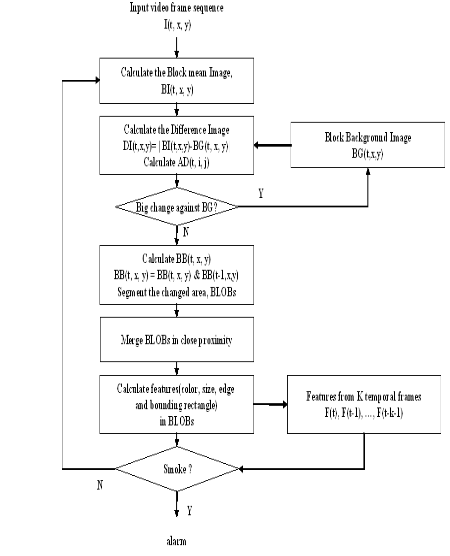
\includegraphics[width=0.65\textwidth]{img/proposta-artigo3.png}
		  \caption{Diagrama da proposta.}
		    \label{fig:sar}
		  \end{center}
		\end{figure}
    \end{column}
\end{columns}
\end{frame}

%%%%%%%%%%%%%%%%%%%%%%%%%%%%%%%%%%%

\begin{frame}{\citeonline{Kim2009}}
	\begin{columns}
		\begin{column}{0.50\textwidth}
			\begin{figure}[H]
				\centering
				\begin{center}
				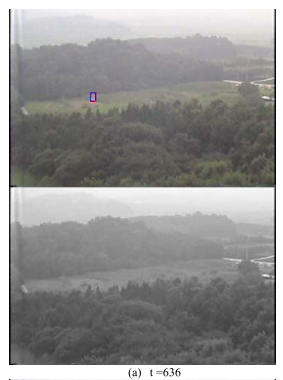
\includegraphics[width=0.75\textwidth]{img/fig2-artigo3-i.png}
				\caption{Resultados I.}
				\label{fig:sar}
				\end{center}
			\end{figure}
		\end{column}
	
		\begin{column}{0.5\textwidth}
			\begin{figure}[H]
				\centering
				\begin{center}
				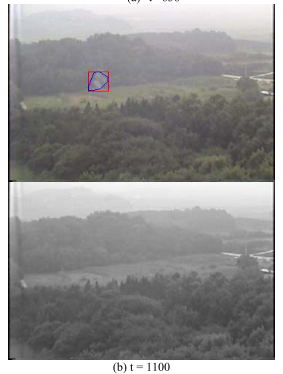
\includegraphics[width=0.75\textwidth]{img/fig2-artigo3-ii.png}
			  \caption{Resultados II.}
				\label{fig:sar}
			  \end{center}
			\end{figure}
		\end{column}
	\end{columns}
\end{frame}

%%%%%%%%%%%%%%%%%%%%%%%%%%%%%%%%%%%

\section{\citeonline{Frizzi2016}}

\begin{frame}{\citeonline{Frizzi2016}}
\begin{columns}
    \begin{column}{0.40\textwidth}
		\begin{itemize}
			\item \textbf{Convolutional Neural Network for Video Fire and Smoke Detection};
			\item Utiliza CNN para detecção de objetos, no caso, chamas;
		\end{itemize}
    \end{column}

    \begin{column}{0.6\textwidth}
		\begin{figure}[H]
		    \centering
		    \begin{center}
		    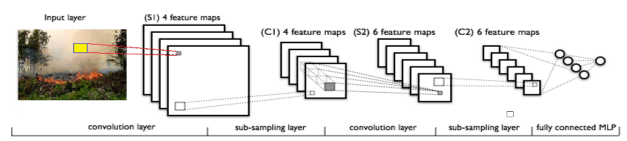
\includegraphics[width=\textwidth]{img/fig2-artigo8.png}
		  \caption{CNN Proposta.}
		    \label{fig:sar}
		  \end{center}
		\end{figure}
    \end{column}
\end{columns}
\end{frame}

%%%%%%%%%%%%%%%%%%%%%%%%%%%%%%%%%%%

\begin{frame}{\citeonline{Frizzi2016}}
	\begin{figure}[H]
		\centering
		\begin{center}
		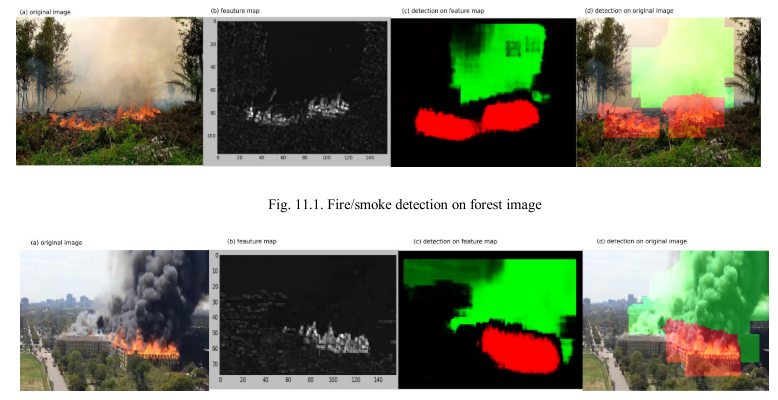
\includegraphics[width=\textwidth]{img/resultados-artigo8.png}
		\caption{Resultados.}
		\label{fig:sar}
		\end{center}
	\end{figure}
\end{frame}

%%%%%%%%%%%%%%%%%%%%%%%%%%%%%%%%%%%

\section{\citeonline{Mutar2018}}

\begin{frame}{\citeonline{Mutar2018}}
\begin{columns}
    \begin{column}{0.40\textwidth}
		\begin{itemize}
			\item \textbf{Smoke Detection Based on Image Processing by Using Grey and Transparency Features};
			\item Acurácia de até 92\%;
			\item Utiliza técnicas como: erosão, dilatação, Transformada de Fourier e Desvio Padrão
		\end{itemize}
    \end{column}

    \begin{column}{0.6\textwidth}
		\begin{figure}[H]
		    \centering
		    \begin{center}
		    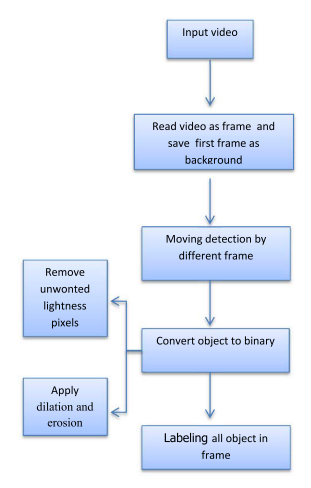
\includegraphics[width=0.51\textwidth]{img/fig2-artigo9.png}
		  \caption{Proposta para detecção de objetos.}
		    \label{fig:sar}
		  \end{center}
		\end{figure}
    \end{column}
\end{columns}
\end{frame}

%%%%%%%%%%%%%%%%%%%%%%%%%%%%%%%%%%%

\begin{frame}{\citeonline{Mutar2018}}
	\begin{columns}
		\begin{column}{0.40\textwidth}
			\begin{figure}[H]
				\centering
				\begin{center}
				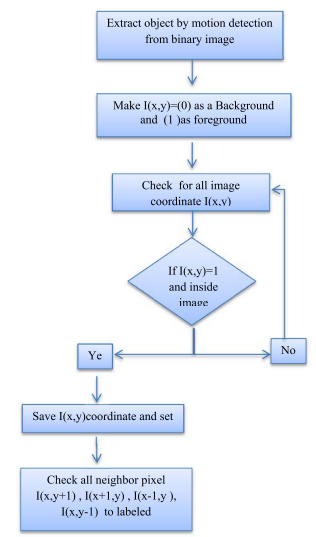
\includegraphics[width=0.65\textwidth]{img/fig5-artigo9.png}
				\caption{Proposta para selecionar regiões.}
				\label{fig:sar}
				\end{center}
			\end{figure}
		\end{column}
	
		\begin{column}{0.6\textwidth}
			\begin{figure}[H]
				\centering
				\begin{center}
				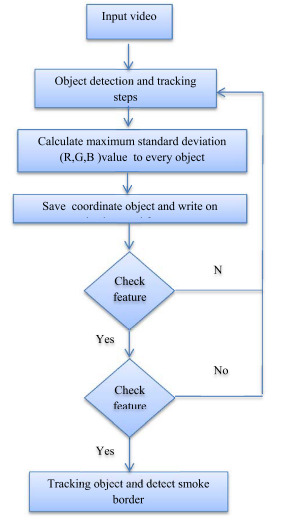
\includegraphics[width=0.45\textwidth]{img/fig10-artigo9.png}
			  \caption{Diagrama da Proposta.}
				\label{fig:sar}
			  \end{center}
			\end{figure}
		\end{column}
	\end{columns}
\end{frame}

%%%%%%%%%%%%%%%%%%%%%%%%%%%%%%%%%%%

\begin{frame}{\citeonline{Mutar2018}}
	\begin{figure}[H]
		\centering
		\begin{center}
		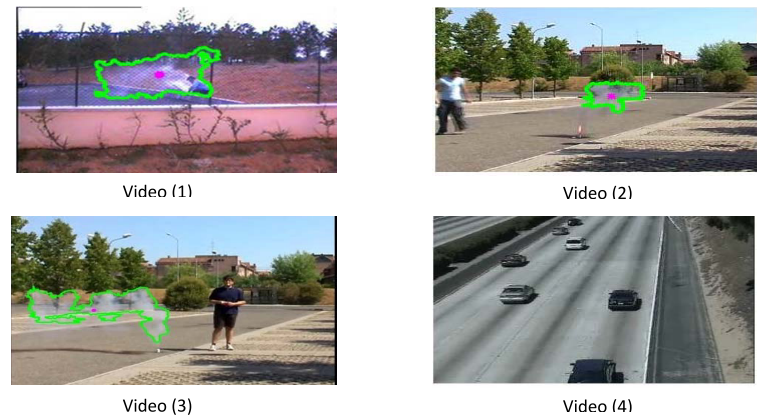
\includegraphics[width=.95\textwidth]{img/resultado1-artigo9.png}
		\caption{Resultado I.}
		\label{fig:sar}
		\end{center}
	\end{figure}
\end{frame}

\begin{frame}{\citeonline{Mutar2018}}
	\begin{figure}[H]
		\centering
		\begin{center}
		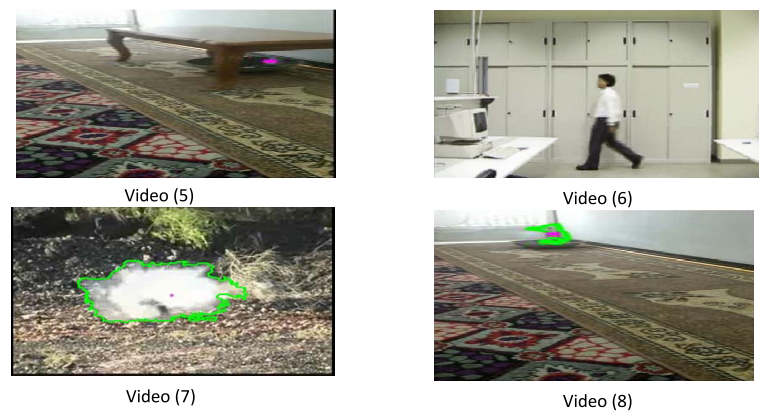
\includegraphics[width=.95\textwidth]{img/resultado2-artigo9.png}
		\caption{Resultado II.}
		\label{fig:sar}
		\end{center}
	\end{figure}
\end{frame}

\begin{frame}{\citeonline{Mutar2018}}
	\begin{figure}[H]
		\centering
		\begin{center}
		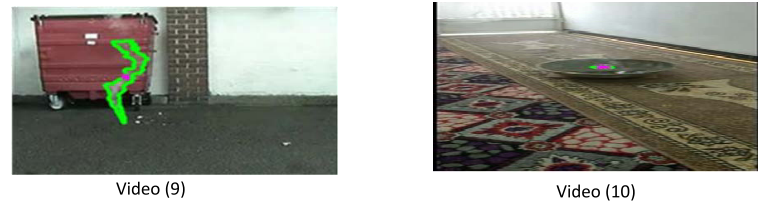
\includegraphics[width=\textwidth]{img/resultado3-artigo9.png}
		\caption{Resultado III.}
		\label{fig:sar}
		\end{center}
	\end{figure}
\end{frame}

%%%%%%%%%%%%%%%%%%%%%%%%%%%%%%%%%%%

\section{Referências Bibliográficas}
\begin{frame}[allowframebreaks]{Referências Bibliográficas}
	\bibliography{smoke-detection}
\end{frame}

%%%%%%%%%%%%%%%%%%%%%%%%%%%%%%%%%%%

\begin{frame}{Agradecimentos}
		\begin{center}
			{\Huge Obrigado pela Atenção!}
		\end{center}
\end{frame}
\end{document}
